\documentclass[conference]{IEEEtran}
\IEEEoverridecommandlockouts
% The preceding line is only needed to identify funding in the first footnote. If that is unneeded, please comment it out.
\usepackage{cite}
\usepackage{amsmath,amssymb,amsfonts}
\usepackage{algorithmic}
\usepackage{graphicx}
\usepackage{textcomp}
\usepackage{xcolor}
\usepackage{listings}
\def\BibTeX{{\rm B\kern-.05em{\sc i\kern-.025em b}\kern-.08em
    T\kern-.1667em\lower.7ex\hbox{E}\kern-.125emX}}
\lstset{language=c++, frame=single, numbers=left, xleftmargin=2em, framexleftmargin=2em, breaklines=true, showstringspaces=false, basicstyle=\scriptsize}
\graphicspath{ {./images/} }

\begin{document}

\title{Parallelizing Sorting Algorithms}

\author{\IEEEauthorblockN{Kevin Alfonso}
\IEEEauthorblockA{\textit{Computer Science, UCF} \\
\textit{Parallel - Group 1}\\
Orlando, Florida \\
kevfonso@knights.ucf.edu}
\and
\IEEEauthorblockN{Gabriella On-Cuen }
\IEEEauthorblockA{\textit{Computer Science, UCF} \\
\textit{Parallel - Group 1}\\
Orlando, Florida \\
Gabriella2024@knights.ucf.edu}
\and
\IEEEauthorblockN{Faiz Ahmed}
\IEEEauthorblockA{\textit{Computer Science, UCF} \\
\textit{Parallel - Group 1}\\
Orlando, Florida \\
faiz@knights.ucf.edu}
\and
\IEEEauthorblockN{Raciel Antela Pardo}
\IEEEauthorblockA{\textit{Computer Science, UCF} \\
\textit{Parallel - Group 1}\\
Orlando, Florida \\
raciel@knights.ucf.edu}
\and
\IEEEauthorblockN{Isaac Munshi}
\IEEEauthorblockA{\textit{Computer Science, UCF} \\
\textit{Parallel - Group 1}\\
Orlando, Florida \\
isaac.p.munshi@knights.ucf.edu}
}

\maketitle

\begin{abstract}
Common sorting algorithms were implemented in parallel to explore the differences in run-time and efficiency between the multi-threaded implementations of the algorithms and the original linear versions. The algorithms tested in this experiment were bubble sort, merge sort, radix sort, insertion sort, selection sort, and quick sort. It has been found that parallelizing sorting algorithms does in fact improve run-time and efficiency. In some algorithms such as bubble sort, the run-times were reduced significantly, while in others such as merge sort and radix sort, the improvements were moderate but still notable.
\end{abstract}

\section{Introduction}
Sorting is used everywhere in computer science, from student projects to enterprise-level software. Oftentimes, this deals with large amounts of data which leads to the sorting taking longer. By rewriting popular sorting algorithms to take advantage of parallelism and multi-threading in a clever way, we can reduce the time it takes to sort large amounts of data at the cost of increased computing power, which is a worthwhile trade due to computers getting more powerful since the days the original sorting algorithms were written and implemented. We will rewrite bubble sort, merge sort, radix sort, insertion sort, selection sort, and quick sort. 

We expect for each sort to take less time as number of threads increase, at least when it comes to large arrays. We also expect for CPU usage to increase as number of threads increase compared to the non-concurrent sorting algorithms.

\section{Problem Statement}
The goal of this project is to analyze the impact of parallelism and multi-threading on sorting algorithms' performance. Specifically, we want to investigate the relationship between the number of threads, sorting time, and CPU usage for each of the six sorting algorithms mentioned above. By comparing the parallelized algorithms' performance to their original implementations, as well as to its own with different number of threads, we can determine the effectiveness of parallelization in reducing sorting time while considering the additional computational resources required. The results of this study can help inform decisions on the use of parallelized sorting algorithms in different scenarios.

\section{Related Work}
This project was done completely independently in terms of code, write-up, evaluation, discussion, etc. No related work was used at any point, but we hope that this project will help others in learning and researching about parallel sorting algorithms.

\section{Technique/Methodology}
We wrote these revised sorting algorithms in C++. We used std::thread to create parallel threads that work on distinct parts of the data simultaneously. Additionally, we used techniques such as lock-free data structures and atomic operations to avoid any race conditions or other synchronization issues that may arise during the parallelization process; this includes the usage of vectors of threads to improve concurrent thread safety and performance as opposed to arrays.

We implemented the normal sorting algorithms and then parallelized them. We tested each sorting algorithm with 1 (not parallel), 2, 4, and 8 threads. We had each thread complete its own sorting work and then merged them together at the end, which typically improves the run-time when compared to doing the same work with only 1 thread.

\subsection{Algorithm to Merge Pieces of Array}
We implemented each concurrent sorting algorithm by splitting the array into multiple smaller subsections and performing a regular sort on each of these subsections before merging them together at the end. To do so we have implemented the merge() function, which we use to merge the smaller sections back together into a full sized array. We call this merge() function shown below in each of our concurrentSort functions. 
\begin{lstlisting}
template <class T>
void merge(T arr[], int start, int mid, int end) {
    int left = start;
    int right = mid + 1;
    int temp[end - start + 1];
    int tempIndex = 0;

    while (left <= mid && right <= end) {
        if (arr[left] < arr[right]) {
            temp[tempIndex] = arr[left];
            left++;
        } else {
            temp[tempIndex] = arr[right];
            right++;
        }
        tempIndex++;
    }

    while (left <= mid) {
        temp[tempIndex] = arr[left];
        left++;
        tempIndex++;
    }

    while (right <= end) {
        temp[tempIndex] = arr[right];
        right++;
        tempIndex++;
    }

    for (int i = start; i <= end; i++) {
        arr[i] = temp[i - start];
    }
}
\end{lstlisting}
\subsection{Bubble Sort}
For our concurrent bubble sort, we first figure out how big each chunk of the array should be based on the array size and number of threads. If the array size is evenly divisible by the number of threads, then the threads handle the same size chunk. Otherwise, the last chunk handles the smaller remainder of data and likely finishes faster. Afterwards, we assign each thread its respective chunk and make it bubble sort it. We join the threads to ensure they are all finished sorting, and then proceed to the final merge step to join together all the chunks of data. This merge is similar to the merge step in merge sort, in that it merges adjacent chunks together, doubling in size every iteration.
\\
% We could not find a way to avoid merging the arrays at the end without sacrificing the correctness of the algorithm or its performance. Running bubble sort for the already sorted chunks would significantly slow down the algorithm. Merging, on the other hand, is much faster since we can take advantage of the already sorted data in the chunks. In practice, this means that concurrent bubble sort is a hybrid implementation of bubble sort and merge sort.

\begin{lstlisting}
template<class T>
void concurrentBubbleSort(T arr[], int n, int numThreads) {
    vector<thread> threads;

    int chunkSize = (int)floor(n / numThreads);

    for (int i = 0; i < numThreads - 1; i++) {
        int start = i * chunkSize;
        int end = start + chunkSize;
        threads.emplace_back(bubbleSort<T>, ref(arr), start, end);
    }
    threads.emplace_back(bubbleSort<T>, ref(arr), (numThreads - 1) * chunkSize, n);

    for (auto &thread: threads) {
        thread.join();
    }

    // Similar to merging in merge sort, but we merge chunks of size chunk_size
    // Doubles the size of the chunks each iteration
    for (int size = chunkSize; size < n; size *= 2) {
        for (int i = 0; i < n - size; i += 2 * size) {
            int left = i;
            int mid = i + size - 1;
            int right = min(i + 2 * size - 1, n - 1);
            merge(arr, left, mid, right);
        }
    }
}
\end{lstlisting}

\subsection{Merge Sort}
Here is part of our implementation for our concurrent Merge Sort. Just like in the normal linear merge sort, we split our array in half recursively. However, we also assign each half to a thread until we run out of threads. Once we run out of threads, we continue splitting the array like normal, then sort, and finally merge. This approach has no waiting or locks and avoids contention. Even though a thread has two sub-threads inside of it, the threads will never fight over accessing data as each thread has its own subset of data and the thread dies after finishing it's job and it passes the array to the parent-thread. Thus, we have successfully parallelized the merge sort function.
\\
\begin{lstlisting}
template <class T>
void concurrentMergeSort(T arr[], int start, int end, int numThreads) {
    if (start < end) {
        int mid = (start + end) / 2;
        
        if (numThreads > 1) {
            vector<thread> threads(2);

            int numThreadsLeft = numThreads / 2;
            int numThreadsRight = numThreads - numThreadsLeft;

            threads[0] = thread(concurrentMergeSort<T>, arr, start, mid, numThreadsLeft);
            threads[1] = thread(concurrentMergeSort<T>, arr, mid + 1, end, numThreadsRight);
            
            for (auto& thread : threads) {
                thread.join();
            }
        } else {
            concurrentMergeSort(arr, start, mid, 1);
            concurrentMergeSort(arr, mid + 1, end, 1);
        }

        merge(arr, start, mid, end);
    }
}
\end{lstlisting}

\subsection{Radix Sort}
Our concurrent radix sort is implemented extremely similarly to the concurrent bubble sort. We split the array into chunks based on the array size and number of threads, assign each thread to radix sort its respective chunk, join the threads, then merge all the chunks together.
\\
\begin{lstlisting}
void concurrentRadixSort(int arr[], int n, int numThreads) {
    vector<thread> threads;

    int chunkSize = (int)floor(n / numThreads);

    for (int i = 0; i < numThreads - 1; i++) {
        int start = i * chunkSize;
        int end = min(start + chunkSize, n);
        threads.emplace_back(radixSort, ref(arr), start, end);
    }
    threads.emplace_back(radixSort, ref(arr), (numThreads - 1) * chunkSize, n);
    
    for (auto &thread: threads) {
        thread.join();
    }

    // Similar to merging in merge sort, but we merge chunks of size chunkSize
    // Doubles the size of the chunks each iteration
    for (int size = chunkSize; size < n; size *= 2) {
        for (int i = 0; i < n - size; i += 2 * size) {
            int left = i;
            int mid = i + size - 1;
            int right = min(i + 2 * size - 1, n - 1);
            merge(arr, left, mid, right);
        }
    }
}
\end{lstlisting}

\subsection{Insertion Sort}
Our concurrent insertion sort is implemented extremely similarly to the concurrent bubble sort and radix sort. We split the array into chunks based on the array size and number of threads, assign each thread to insertion sort its respective chunk, join the threads, then merge all the chunks together.
\\
\begin{lstlisting}
void concurrentInsertionSort(int arr[], int n, int num_threads) {
    vector<thread> threads;

    int chunkSize = (int)floor(n / num_threads);

    for (int i = 0; i < num_threads-1; i++) {
        int start = i * chunkSize;
        int end = min(start + chunkSize, n);
        threads.emplace_back(insertionSort, ref(arr), start, end - 1);
    }
    threads.emplace_back(insertionSort, ref(arr), (num_threads - 1) * chunkSize, n - 1);    

    for (auto &thread : threads) {
        thread.join();
    }
    
    // Similar to merging in merge sort, but we merge chunks of size chunkSize
    // Doubles the size of the chunks each iteration
    for (int size = chunkSize; size < n; size *= 2) {
        for (int i = 0; i < n - size; i += 2 * size) {
            int left = i;
            int mid = i + size - 1;
            int right = min(i + 2 * size - 1, n - 1);
            merge(arr, left, mid, right);
        }
    }
}
\end{lstlisting}

\subsection{Selection Sort}
For our selection sort approach, we first split the array into chunks based on the number of threads and the size of the array. We then create numThreads - 1 threads, each of which sorts a chunk of the array. The last thread sorts the remaining elements of the array that are not covered by the other threads. Lastly, we merge the sorted subarrays. We do this by iteratively merging subarrays of increasing size, starting with the chunk size and doubling the size each iteration. Similarly to the previous concurrent sorting algorithms, the merging step ensures that the entire array is sorted correctly.
\\
\begin{lstlisting}
void concurrentSelectionSort(int arr[], int n, int numThreads) {
    vector<thread> threads;

    int chunkSize = (int)floor(n / numThreads);

    for (int i = 0; i < numThreads - 1; i++) {
        int start = i * chunkSize;
        int end = min(start + chunkSize, n);
        threads.emplace_back(selectionSort, ref(arr), start, end - 1);
    }
    threads.emplace_back(selectionSort, ref(arr), (numThreads - 1) * chunkSize, n - 1);
    
    for (auto &thread : threads) {
        thread.join();
    }

    // Similar to merging in merge sort, but we merge chunks of size chunkSize
    // Doubles the size of the chunks each iteration
    for (int size = chunkSize; size < n; size *= 2) {
        for (int i = 0; i < n - size; i += 2 * size) {
            int left = i;
            int mid = i + size - 1;
            int right = min(i + 2 * size - 1, n - 1);
            merge(arr, left, mid, right);
        }
    }
}
\end{lstlisting}

\subsection{Quick Sort}
Our quick sort follows a similar approach as our previous concurrent sorts. We divide the array into chunks, sort each chunk using threads, and then merge the sorted chunks together.
\\
\begin{lstlisting}
void concurrentQuickSort(int arr[], int n, int numThreads) {
    vector<thread> threads;

    int chunkSize = (int)floor(n / numThreads);

    for (int i = 0; i < numThreads - 1; i++) {
        int start = i * chunkSize;
        int end = min(start + chunkSize, n);
        threads.emplace_back(quickSort, ref(arr), start, end - 1);
    }
    threads.emplace_back(quickSort, ref(arr), (numThreads - 1) * chunkSize, n - 1);
    
    for (auto &thread : threads) {
        thread.join();
    }

    // Similar to merging in merge sort, but we merge chunks of size chunkSize
    // Doubles the size of the chunks each iteration
    for (int size = chunkSize; size < n; size *= 2) {
        for (int i = 0; i < n - size; i += 2 * size) {
            int left = i;
            int mid = i + size - 1;
            int right = min(i + 2 * size - 1, n - 1);
            merge(arr, left, mid, right);
        }
    }
}
\end{lstlisting}

\section{Evaluation}
While some of the sorts were implemented with generics, we only tested with randomly generated arrays of integers with a predetermined size. Every sort was given the same randomly sorted arrays. After each sort, we checked to see if each sort resulted in a sorted array to ensure its validity. Before and after each sort, we collected timing and CPU data to measure time and CPU Usage. Time was measured std::chrono's high resolution clock and cast to microseconds for both accuracy and readability. CPU busy time was measured with linux's rusage, and CPU Usage, as a percent, was calculated as $(busy time) / (elapsed time) / (number of cores) * 100$. To evaluate our sorts, we outputted all the data collected for each run (sort name, array size, time taken, CPU usage, and number of threads used) into a table through standard output for easy viewing by anyone who runs the code. We also outputted it as a CSV file in the format of “Sort Name,Array Size,Time Taken,CPU Usage,Number of Threads Used”. We then used this to make charts and plots from the data in a Python Jupyter notebook, allowing us to easier visualize relationships between all the variables. For that we used Pandas, Matplotlib, and Seaborn. We plotted Time Taken vs Array Size and CPU Usage vs Array Size, with number of threads as the third variable represented by color.

\subsection{Miscellaneous Functions}
As mentioned before, we checked if sorts actually produced a sorted array to ensure validity after each benchmark. This is how it was done.
\begin{lstlisting}
// Mainly for debugging purposes
void isSorted(int arr[], int arrSize, string arrName = "Array") {
    bool isSorted = true;
    for (int i = 0; i < arrSize - 1; i++) {
        if (arr[i] > arr[i + 1]) {
            isSorted = false;
            cout << arrName << " is not sorted" << endl;
            cout << "arr[" << i << "] = " << arr[i] << " and arr[" << i + 1 << "] = " << arr[i + 1] << endl << endl;
            // return;
        }
    }
    if (isSorted) cout << arrName << " is sorted" << endl << endl;
}
\end{lstlisting}
Additionally, CPU Usage was calculated with our code with the following function.
\begin{lstlisting}
// Calculates CPU Usage as busy time / elapsed time * 100 / number of cores
double calculateCpuUsage(struct rusage startUsage, struct rusage endUsage, double elapsedTime) {
    double start = (double) startUsage.ru_utime.tv_sec + (double) startUsage.ru_utime.tv_usec / 1000000.0
                 + (double) startUsage.ru_stime.tv_sec + (double) startUsage.ru_stime.tv_usec / 1000000.0;
    double end = (double) endUsage.ru_utime.tv_sec + (double) endUsage.ru_utime.tv_usec / 1000000.0
               + (double) endUsage.ru_stime.tv_sec + (double) endUsage.ru_stime.tv_usec / 1000000.0;
    double cpuUsage = (end - start) * 100.0 / elapsedTime / thread::hardware_concurrency();
    return cpuUsage;
}
\end{lstlisting}
\subsection{Time Taken Charts}
We used Python Jupyter notebook to take in the data for each of our sorts to create charts displaying the data in an easy to comprehend manner. Here is the Python code we used to create charts for each of our sorts comparing the execution times for different numbers of threads at multiple different array sizes. Note that the y-axis was plotted on a logarithmic scale.
\lstset{language=python, frame=single, numbers=left, xleftmargin=2em, framexleftmargin=2em, breaklines=true, showstringspaces=false, basicstyle=\scriptsize}
\begin{lstlisting}
# Get a list of the unique sort names
sorts = df['Sort Name'].unique()

# Loop over each sort
for sort in sorts:
    
    # Filter the data for the current sort
    data = df[df['Sort Name'] == sort]

    # Set up the figure for the sort
    plt.figure(figsize=(15, 6))

    # Plot the time taken by the sort for each array size, with the number of threads used as the hue
    sns.barplot(x='Array Size', y='Time Taken', hue='Number of Threads Used', data=data)

    # Set the title, legend, and axis labels
    plt.title(f'Time Taken by {sort} for Different Array Sizes')
    plt.legend(title='Number of Threads Used', loc='upper left')
    plt.xlabel('Array Size (# of Elements)')
    plt.ylabel('Time Taken (us)')
    
    # Set the y axis to be logarithmic to better show the differences in time taken 
    # Some sorts takes so long that the other array sizes are not visible on the graph otherwise
    plt.yscale('log')

    # Show the plot
    plt.show()
\end{lstlisting}

\subsection{CPU Usage Charts}
In addition to the time taken charts, we also used Python Jupyter notebook to take in the data for each of our sorts to create charts displaying the CPU usage of our concurrent sorts in an easy to comprehend manner. Here is the Python code we used to create charts for each of our sorts comparing the CPU usage for different numbers of threads at multiple different array sizes. 

\begin{lstlisting}
# Get a list of the unique sort names
sorts = df['Sort Name'].unique()

# Loop over each sort
for sort in sorts:
    
    # Filter the data for the current sort
    data = df[df['Sort Name'] == sort]

    # Set up the figure for the sort
    plt.figure(figsize=(15, 6))

    # Plot the CPU usage of the sort for each array size, with the number of threads used as the hue
    sns.barplot(x='Array Size', y='CPU Usage', hue='Number of Threads Used', data=data)

    # Set the title, legend, and axis labels
    plt.title(f'CPU Usage of {sort} for Different Array Sizes')
    plt.legend(title='Number of Threads Used', loc='upper left')
    plt.xlabel('Array Size (# of Elements)')
    plt.ylabel('CPU Usage (%)')

    # Show the plot
    plt.show()
\end{lstlisting}

\subsection{Bubble Sort}
Bubble sort was the golden child of showing relationships in our data. It has a run-time of $\mathcal{O}(n^2)$. It very clearly shows that at some point between 100 and 1000 for the array size, bubble sort benefits more from multi-threading through time saving than it wastes time from the thread creation and management overhead.
Regarding the CPU usage, starting somewhere between 10,000 and 100,000 elements, there begins a linear relationship between the increase in number of threads and increase in CPU usage. It shows in an almost exact perfect relationship that multithreading puts more strain on the CPU compared to sequential programming (doubling threads means doubling CPU usage percent). However, as mentioned in the introduction, this is often worth it due to constantly improving computing power mixed with a need for quickly sorted data.
\\\\
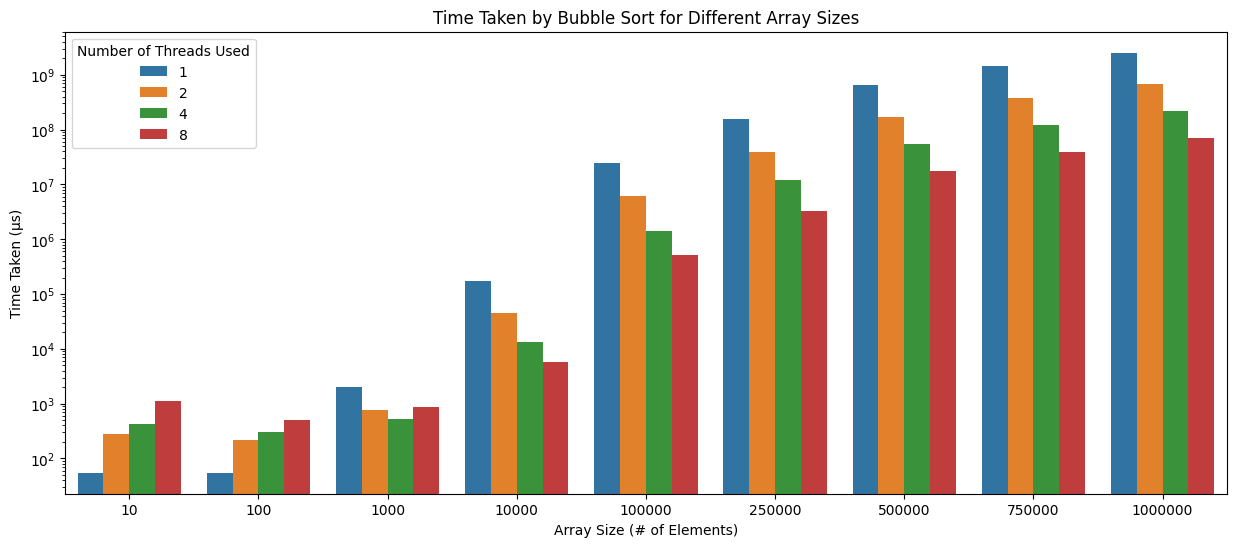
\includegraphics[width=3.5in]{BubbleSortTimeTaken.png}
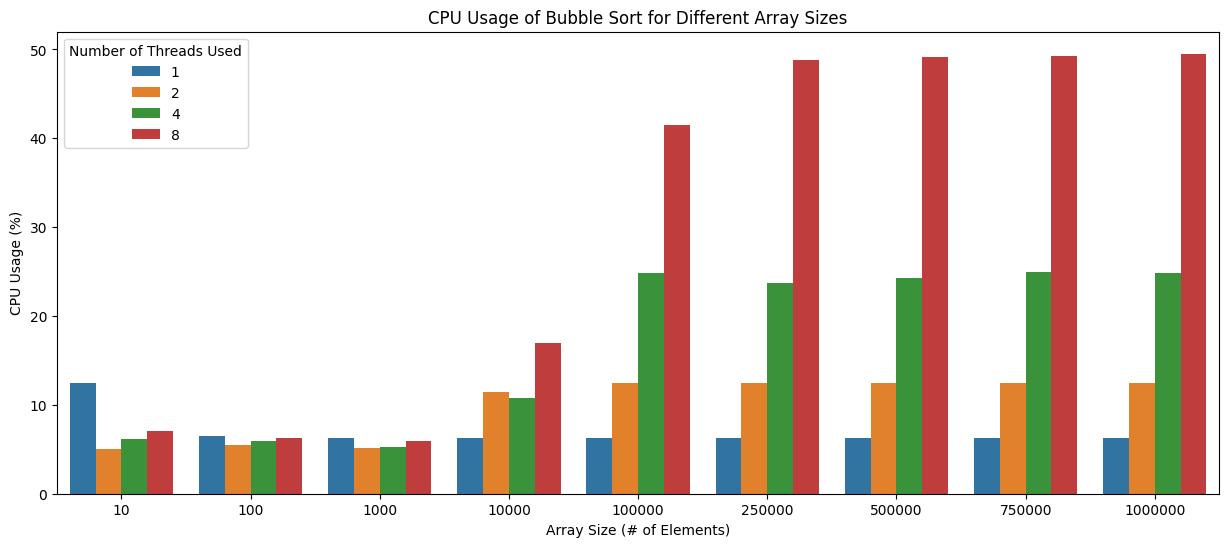
\includegraphics[width=3.5in]{BubbleSortCPUUsage.png}

\subsection{Merge Sort}
Merge sort is so fast with its average run-time of $\mathcal{O}(n\log{}n)$ compared to bubble sort that the point for when multi-threading becomes beneficial is between 1000 and 10000 for the array size. Its improved run-time also means it has less room for improvement as we double the amount of threads, especially compared to bubble sort.
Starting somewhere between 100,000 and 250,000 elements, there begins a linear relationship between the increase in number of threads and increase in CPU usage. Merge Sort's CPU usage relationship is slightly less apparent than bubble sort's, but it can be seen that certain array sizes indeed raise CPU usage as thread count is increasing, pointing more towards the measurable cost of thread overhead. 
\\\\
\includegraphics[width=3.5in]{MergeSortTimeTaken.png}
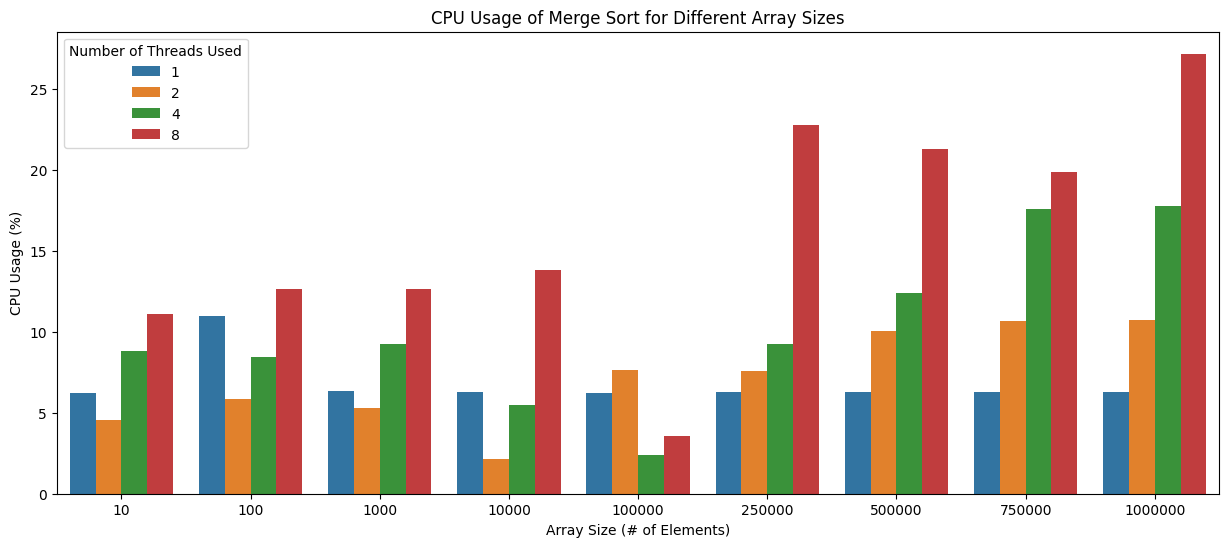
\includegraphics[width=3.5in]{MergeSortCPUUsage.png}

\subsection{Radix Sort}
Radix sort, with an average run-time of $\mathcal{O}(d*(n+b)$ where d is the number of digits of the largest number in the array and b is the base size (in this case 10), benefited the least from an increasing number of threads. Our results show that the best approach is to use 4 threads when your array is 10,000 elements or more. 
For datasets of size 10,000 or more, run-time was improved from 1 to 2 threads, the improvement from 2 to 4 threads was small, and there was little to no improvement from 4 to 8 threads. In fact, the 8-thread approach used significantly more CPU resources making it an over-all worse approach than the 4-thread approach! Also interestingly is that in almost every array size, the CPU usage for 4 threads was smaller than the 2-thread approach. The linear relationship between increase in thread number and increase in CPU usage starts somewhere between 250,000 and 500,000 elements, which is significantly higher than most of the other sorts, indicating that radix sort has a less predictable relationship between multithreading and CPU usage overall. 
\\\\
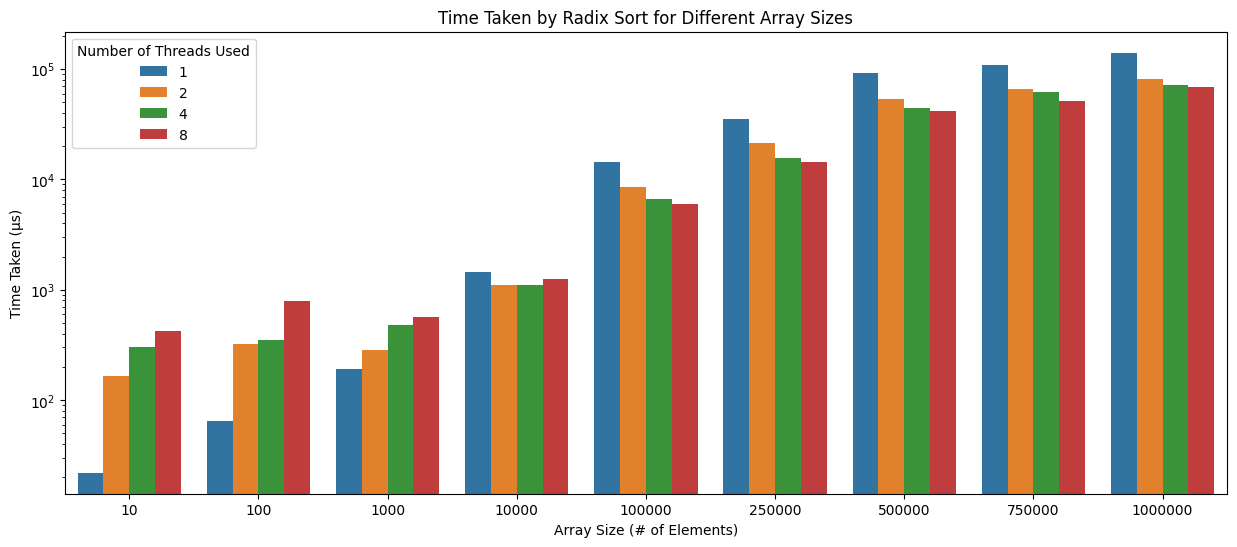
\includegraphics[width=3.5in]{RadixSortTimeTaken.png}
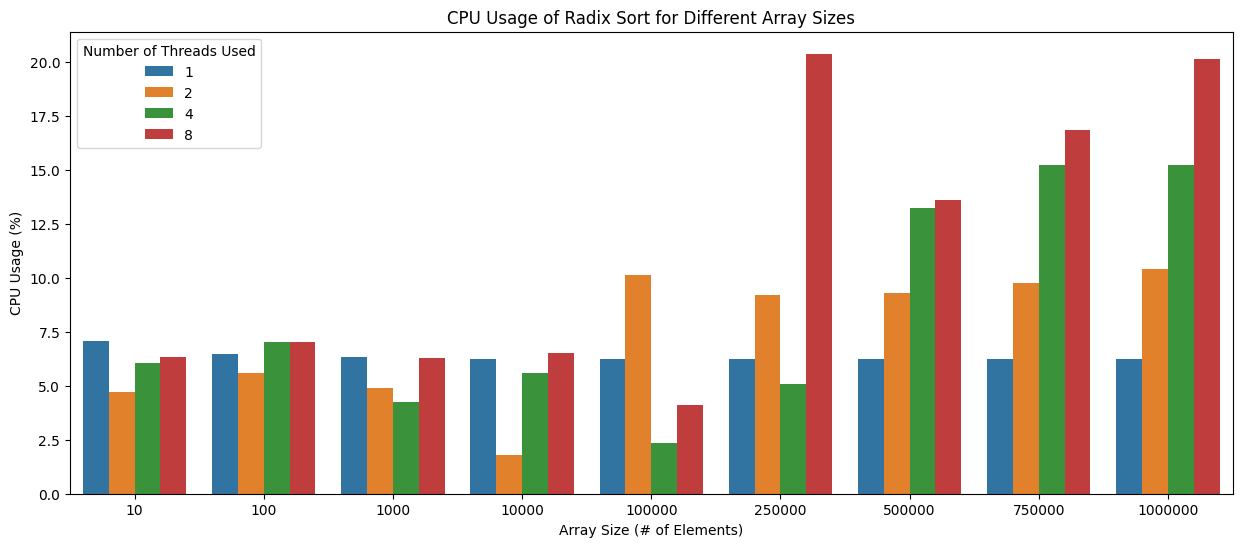
\includegraphics[width=3.5in]{RadixSortCPUUsage.png}

\subsection{Insertion Sort}
Insertion sort showed noticeable benefits when multi-threading, likely due to the fact that its run-time is on the slower side, with an average run-time of $\mathcal{O}(n^2)$. Like bubble sort, it very clearly shows that at some point between 100 and 1,000 for the array size, although likely at the higher end of this range, insertion sort benefits more from multi-threading through time saving than it wastes time from the thread creation and management overhead. At the higher array sizes, multi-threading leads to higher CPU usage. Starting somewhere between 10,000 and 100,000 elements, insertion sort starts to develop a linear relationship between increase in thread number and increase in CPU usage. Like bubble sort, at higher array sizes, there is an almost perfect correlation between thread count and CPU usage. If you double the number of threads, you double the CPU usage. Therefore we can say there is a very strong and consistent relationship between thread count and CPU usage for insertion sort at higher array sizes. 
\\\\
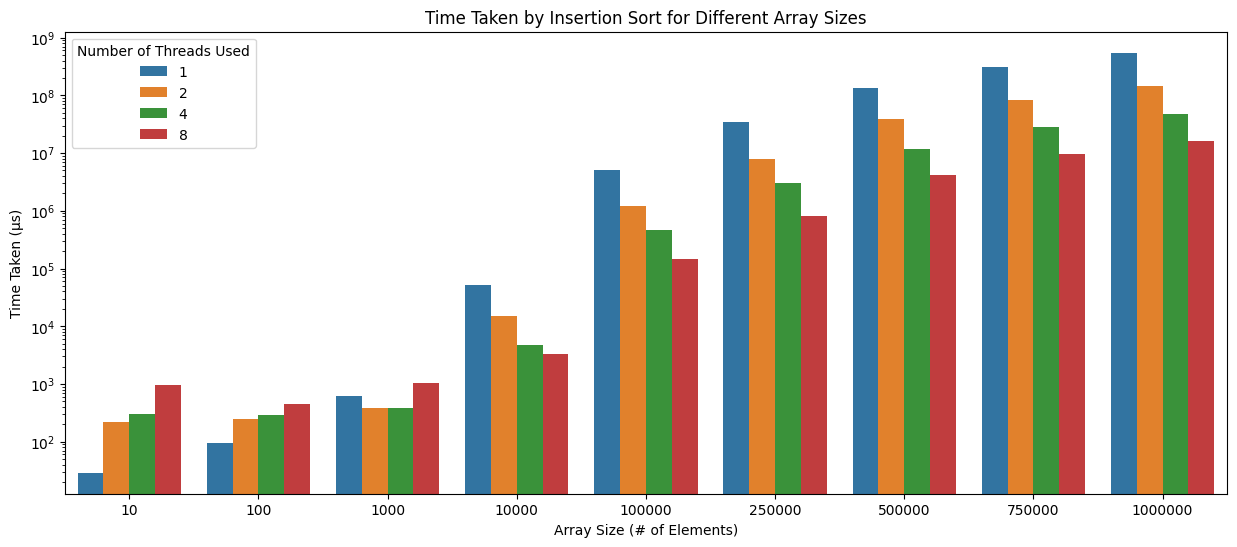
\includegraphics[width=3.5in]{InsertionSortTimeTaken.png}
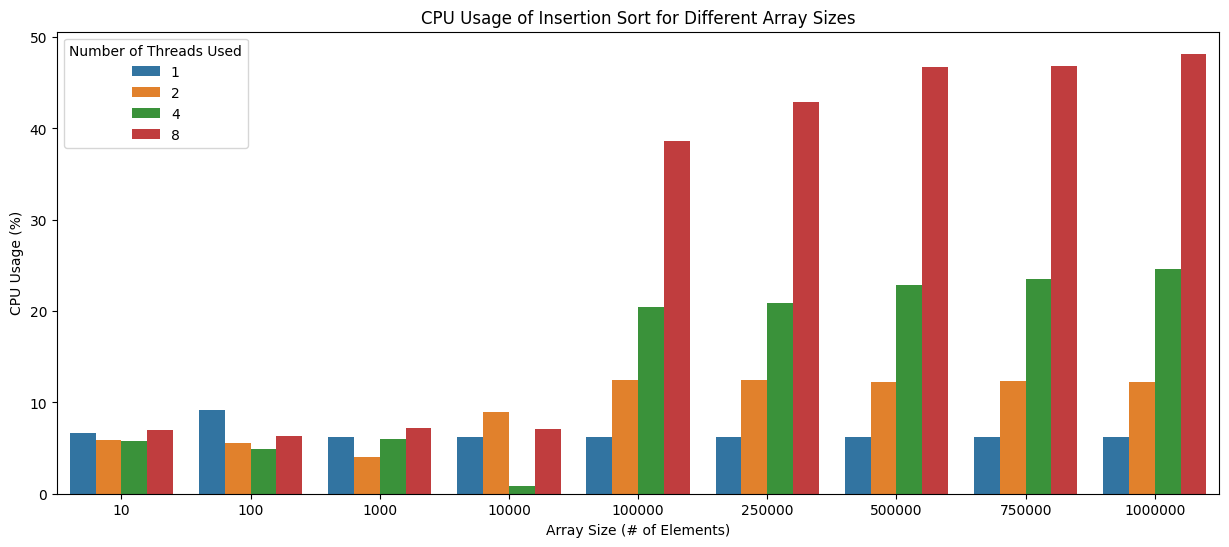
\includegraphics[width=3.5in]{InsertionSortCPUUsage.png}

\subsection{Selection Sort}
Selection sort, with its average run-time of $\mathcal{O}(n^2)$, noticeably benefited from an increase in thread count. Our results show that it is most efficient when using 8 threads for array elements equaling 10,000 or more. We can also see that the decrease in time taken follows a linear pattern for more than 10,000 elements. As we go lower in element count, the overhead of threading outweighs any benefit parallelization brings. Starting somewhere between 10,000 and 100,000 elements, there begins a linear relationship between the increase in number of threads and increase in CPU usage. The CPU usage doubles as the thread count doubles. However, for lower than 10,000 elements, the CPU usage remains somewhat the same indicating that multi-threading is not taking enough advantage of the CPU processing power compared to higher element counts.
\\\\
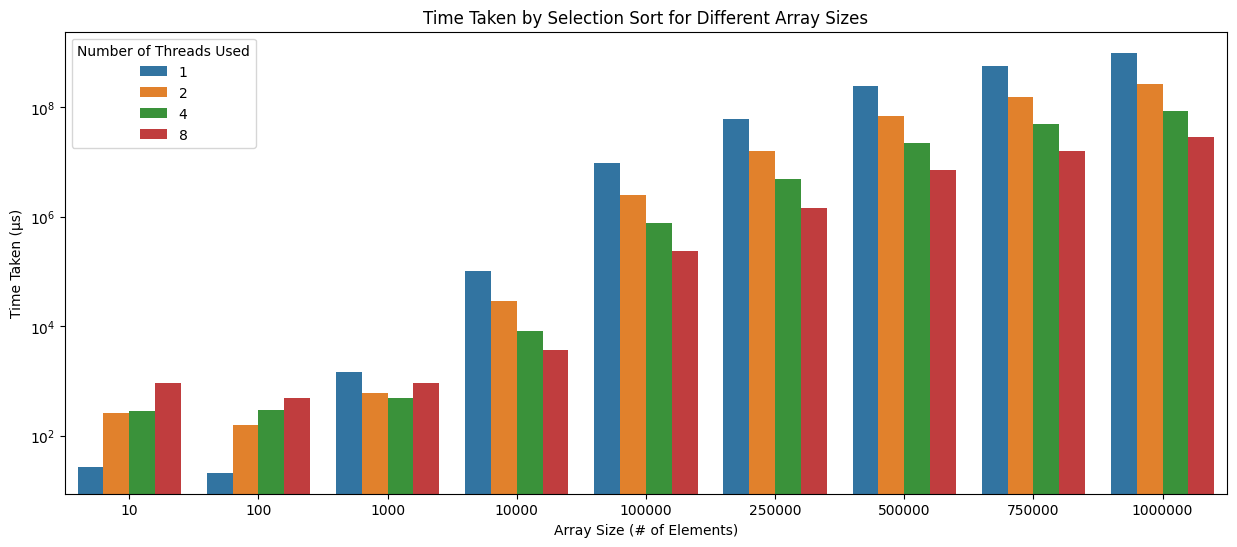
\includegraphics[width=3.5in]{SelectionSortTimeTaken.png}
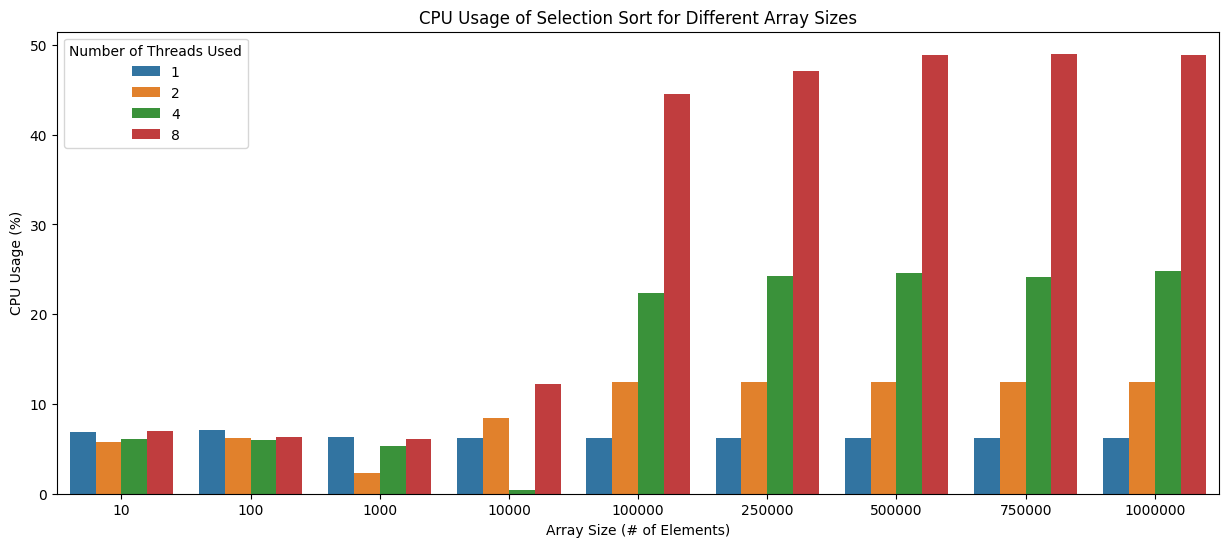
\includegraphics[width=3.5in]{SelectionSortCPUUsage.png}

\subsection{Quick Sort}
Quick sort benefits from multithreading in terms of time taken starting between 1000 and 10000 elements, but the benefits are much more noticeable at even larger array sizes. This is due to quick sort's fast run-time, with an average run-time of $\mathcal{O}(n\log{}n)$. The CPU usage also further shows that multithreading shows a more linear relationship as array size increases. This linear relationship between the increase in number of threads and increase in CPU usage starts somewhere between 500,000 and 750,000 elements. For lower array sizes, they are pretty similar. For bigger array sizes, 4 threads tended to have more CPU usage than 8 threads surprisingly.
\\\\
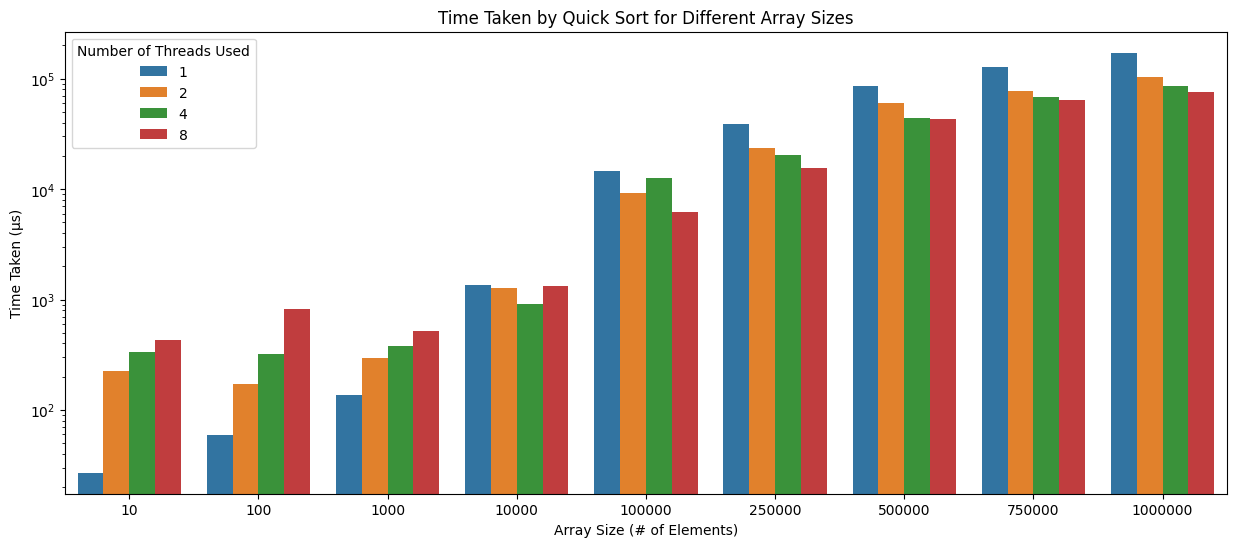
\includegraphics[width=3.5in]{QuickSortTimeTaken.png}
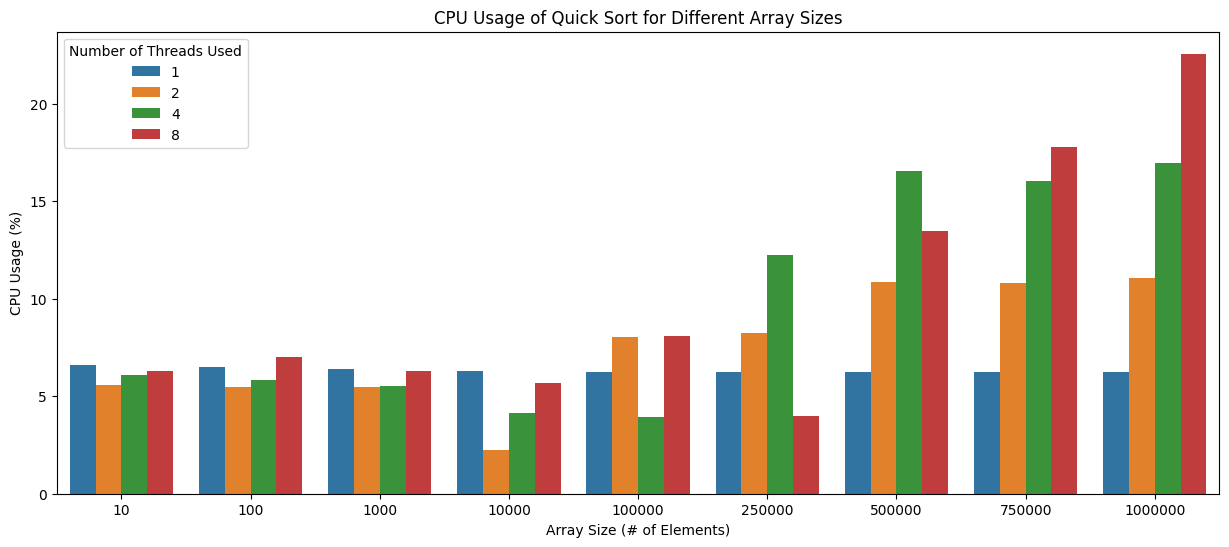
\includegraphics[width=3.5in]{QuickSortCPUUsage.png}

\section{Discussion}
% The implementations our team designed showed great results, but there are many ways to implement concurrency in sorting algorithms. For example, researchers could try implementing concurrency in sorts without needing a merge step at the end by having the merge be done "along the way" as the sort is being completed, and that could possibly speed it up over one large merge step. In the future, other researchers can take different approaches to parallelizing the sorting methods addressed in our paper and compare results. There are always more ways to assign jobs to threads. Or, they can take our research and apply it to new methods we have not covered.

Our team designed and implemented several sorting algorithms with multi-threading to evaluate their performance in terms of time taken, CPU usage, number of threads used, and array size. Our results demonstrate that multi-threading can significantly improve the performance of sorting algorithms for larger array sizes. However, the optimal array size for multi-threading varied depending on the sorting algorithm and system specifications.
\\\\
Our study focused on six common sorting algorithms: bubble sort, merge sort, radix sort, insertion sort, selection sort, and quick sort. Each algorithm had its own unique characteristics and performance trade-offs. For example, bubble sort showed a clear point where multi-threading became beneficial, which was between 100 and 1000 for the array size, while radix sort showed the least benefit from multi-threading, with the best approach being to use four threads when the array size was 10,000 or more.
\\\\
Moreover, our study highlighted the importance of carefully considering the overhead of thread creation and management when deciding whether to use multi-threading. For some algorithms, such as bubble sort and insertion sort, the benefits of parallel processing outweighed the cost of overhead, while for others, such as radix sort, the cost of overhead was too high to make multi-threading worthwhile, at least for higher thread counts.
\\\\
Our project faced some challenges throughout the development process. Our original bubble sort implementation was faulty, which was fixed by changing the bounds of its normal version's inner loop. Merging of arrays sometimes produced arrays not sorted at chunk bounds, which was fixed by changing from linear merging to merge-sort like merging shown in our code above. Some parallel sorts did not work when array size was not evenly divisible by the number of chunks, which was fixed by making the last thread handle the remainder of data.
\\\\
Some relationships were observed throughout all our evaluation. The faster sorts require a larger array for multithreading to become worth it. CPU Usage has a more linear relationship as array size increases.
\\\\
One potential area for future research is exploring different ways to implement concurrency in sorting algorithms, such as implementing concurrency in sorts without needing a merge step at the end. One such example we considered was using all threads to operate on one array and utilizing locks to avoid contention. This skips the steps of breaking the array into chunks and the final merge step. Furthermore, we did not parallelize the final merge step, but future researchers could do this to see noticeable improvements in the run-time of multi-thread sorting. These are just a few approaches that researchers could take to avoid the thread overhead and there are many more improvements to discover. To improve run-time in a different manner, researchers could also investigate new ways of assigning jobs to further bring down the overhead run-time cost. Lastly, researchers could augment our implementations or apply them to new sorting methods that we have not covered.

\section{Conclusion}
In conclusion, our study demonstrated that implementing common sorting algorithms with multi-threading can improve their performance in terms of time taken for sorting to complete, although this is only worth it for larger array sizes. The specific size depends on the type of sort and specifications of the system doing the sorting. Our study focused on six common sorting algorithms, with each having unique characteristics and performance trade-offs. Our findings highlight the importance of carefully considering the overhead of thread creation and management when deciding whether to use multi-threading.
\\\\
Our results can be applied to real-world scenarios, such as large-scale data processing or optimizing computer systems. For instance, if sorting a large dataset, it may be worth the overhead of multi-threading to improve performance, whereas for smaller datasets, the overhead may outweigh the benefits of parallel processing.
\\\\
However, our study is not without limitations. The choice of sorting algorithms may have biased our results, and we used a specific hardware and software setup for testing. Future research could investigate additional sorting algorithms and use different hardware and software setups to validate our findings.
\\\\
In summary, our study contributes to the growing body of research on concurrency in sorting algorithms, and our results have practical implications for improving the performance of sorting algorithms in real-world scenarios.

\end{document}
